\chapter{Định nghĩa và một số kí hiệu}
Trong chương này, chúng ta sẽ đưa ra định nghĩa chính tắc cho lớp các bài toán định tuyến xe. Các định nghĩa này được xây dựng theo ngôn ngữ của lý thuyết đồ thị được đưa ra bởi Toth (2002) \cite{toth2002vehicle}. 

Các bài toán được mô tả thuộc lớp VRP (\textit{vehicle routing problem}) bao gồm \textit{định tuyến xe với ràng buộc tải trọng} - CVRP (\textit{capacited VRP}), \textit{định tuyến xe với ràng buộc khung thời gian} - VRPTW (\textit{VRP with time windows}), \textit{định tuyến xe với lấy và giao hàng} - VRPPD (\textit{VRP with pickup and delivery}).

\begin{figure}[H] % places figure environment here   
  \centering % Centers Graphic
  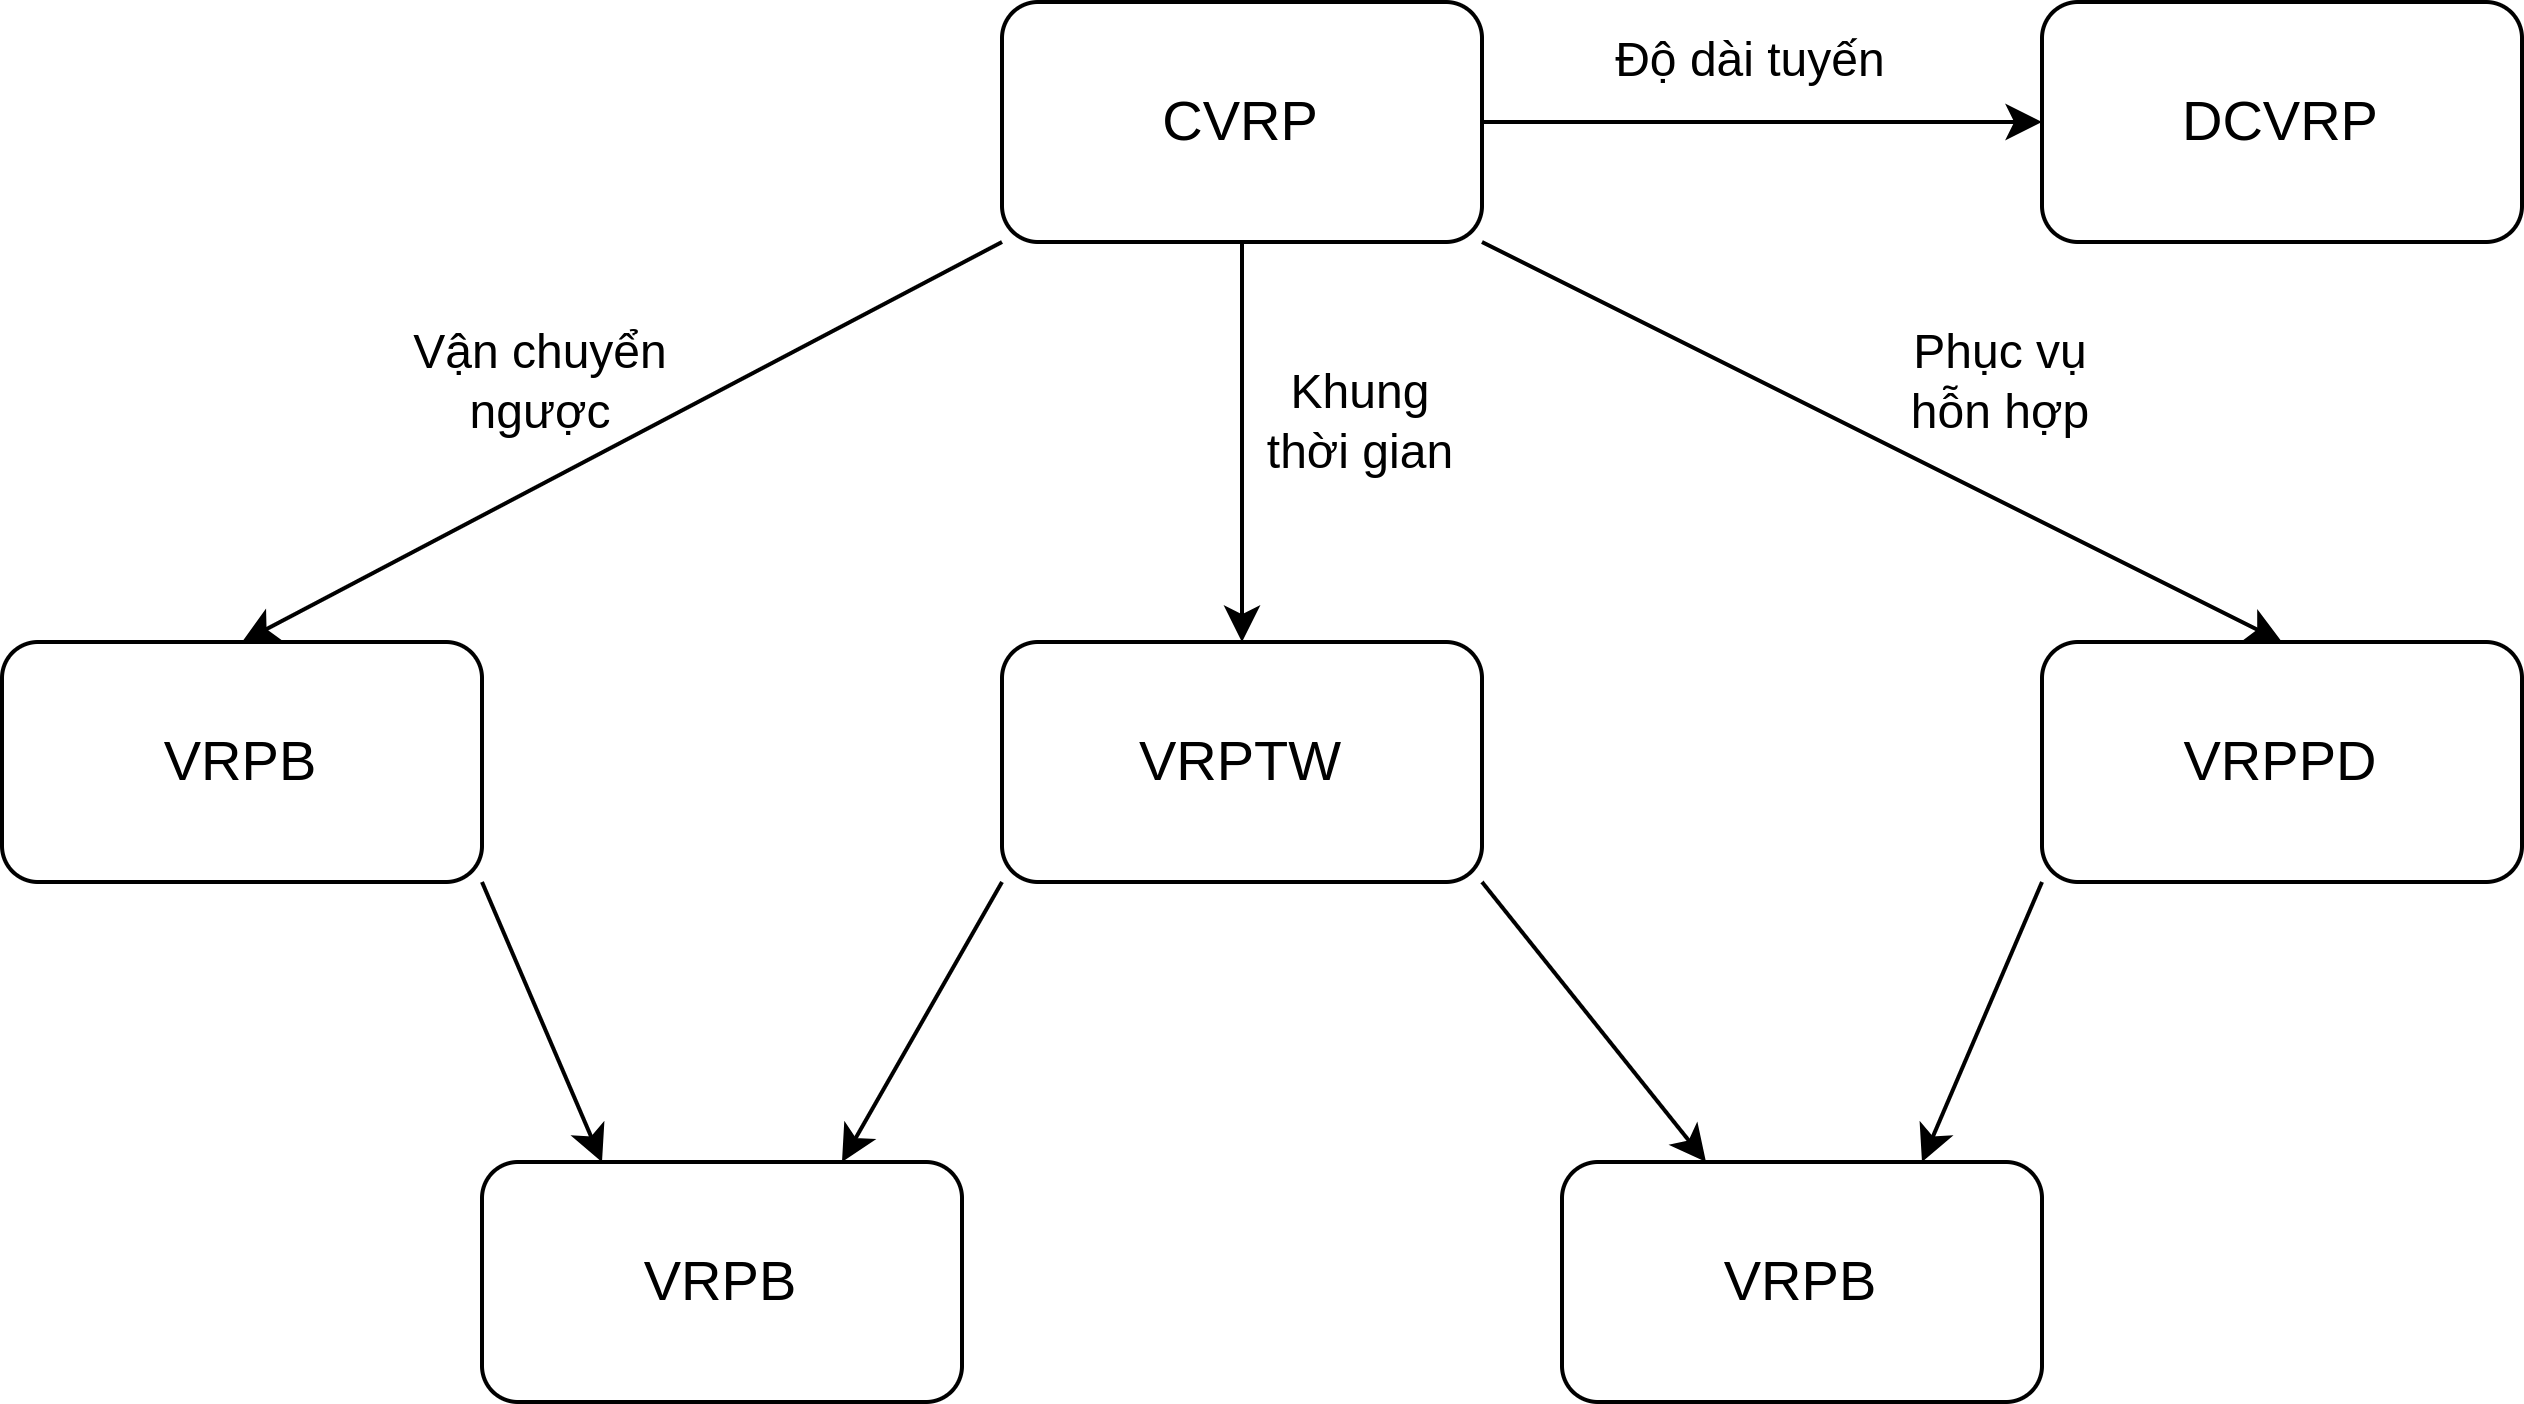
\includegraphics[width=0.8\textwidth]{figures/vrp.png} 
  \caption{Các bài toán, biến thể của VRP} % Creates caption underneath graph
  \label{fig:fg_01}
\end{figure}

\section{CVRP}

Trước hết ta xem xét mô hình cho bài toán \textit{nguyên bản}: \textit{bài toán định tuyến xe với ràng buộc tải trọng}. Một cách tự nhiên, tại sao không phải là VRP (không ràng buộc)? Bạn sẽ thấy rằng nếu không có bất kì ràng buộc nào thì một xe có thể phục vụ tất cả các yêu cầu và bài toán VRP sẽ suy biến về TSP (\textit{travelling salesman problem}). Ít nhất ràng buộc về tải trọng là thực tế và giữ cho mỗi xe chỉ phục vụ được một số yêu cầu nhất định (trong trường hợp số yêu cầu không quá nhỏ cũng như tải trọng của xe là quá lớn). 


Gọi $G=(V,A)$ là một độ thị đầy đủ với $V=\{ 0, ..., n \}$ là tập nút và $A$ là tập các cung. Các nút $i=1,...,n$ đại diện cho các yêu cầu hay khách hàng cần phục vụ, nút $0$ là kho hàng. 

Một số không âm được gọi là chi phí $c_{ij}$ đại diện cho mỗi cung $(i,j) \in A$. Nói cách khác $c_{ij}$ là  chi phí cần bỏ ra để di chuyển từ đỉnh $i$ tới nút $j$. Trong bài toán này và hầu hết các bài toán định tuyến ta không định nghĩa canh $(i,i)$ nên có thể gán $c_{ii} = \infty$ với $i \in V$.

Nếu đồ thị là có hướng thì ma trận chi phí $C$ là bất đối xứng, khi đó ta có bài toán CVRP bất đối xứng ACVRP (\textit{asymetric CVRP}). Ngược lại nếu $c_{ij} = c_{ji}$ với mọi $(i,j) \in A$ ta có bài toán CVRP đối xứng SCVRP (\textit{symetric CVRP}) và các cung của $A$ được thay thế bằng tập cách cạnh vô hướng $E$. Với một cạnh $e \in E$, gọi $\alpha(e)$ và $\beta(e)$ là nút bắt đầu và kết thúc của cạnh. 

Đồ thị $G$ phải là đồ thị kết nối mạnh và nhìn chung ta giả thiết đồ thị $G$ là đầy đủ. Với một nút $i$, gọi $\Delta^+(i)$ là tập ra của $i$ (\textit{forward star}), được định nghĩa là tập các nút $j$ mà cung $(i,j) \in A$, nói cách khác đây là tập các nút có thể tiếp cận trực tiếp từ nút $i$. Tương tự như vậy, $\Delta^-{i}$ là tập vào của $i$ (\textit{backward star}), được định nghĩa là tập các nút $j$ mà cung $(j,i) \in A$ hay là tập các nút tiếp cận trực tiếp tới nút $i$. Với một tập nút con $S \subseteq V$, gọi $\delta(S)$ và $E(S)$ là tập các cạnh $e \in E$ chỉ có một hoặc cả hai đầu mút thuộc $S$. Để thuận tiện khi xét một nút $i \in V$, ta viết $\delta(i)$ thay cho $\delta(\{i\})$.

Trong hầu hết các bài toán thực tế, ma trận chi phí thỏa mãn bất đẳng thức tam giác 
\begin{equation}
    c_{ij} + c_{jk} \geq c_{ik} \quad \forall i,j,k \in V
\end{equation}
Nói cách khác việc đi trực tiếp từ nút $i$ tới nút $j$ luôn tốn ít chi phí hơn là đi gián tiếp. Với nhiều thuật toán, bất đẳng thức tam giác là điều kiện cần, điều này có thể được đảm bảo bằng cách thêm một đại lượng dương lớn (hợp lý) vào chi phí của mỗi cung. Ta chú ý thêm rằng nếu chi phí của mỗi cung thuộc đồ thị bằng với chi phí của đường đi ngắn nhất giữa hai đầu mút của cung thì mà trận chi phí thỏa mãn bất đẳng thức tam giác.

Trong nhiều trường hợp, tập các nút nằm trên một mặt phẳng, vị trí của chúng được cho bởi tọa độ và chi phí $c_{ij}$ của mỗi cung $(i,j) \in A$ là khoảng cách Euclide giữa hai điểm ứng với nút $i$ và $j$. Khi đó, ma trận chi phí là đối xứng và thỏa mãn bất đẳng thức tam giác. Bài toán này được gọi là \textit{Euclidian} SCVRP.

Mỗi khách hàng $i$ có một nhu cầu (về tải trọng) là $d_i$ và nhu cầu của kho $d_0=0$. Với một tập nút $S \subseteq V$, ta kí hiệu $d(S) = \sum_{i \in S} d_i$ là tổng nhu cầu của tập.

Một tập hợp $K$ đại diện cho các xe, mỗi xe có tải trọng $C$ và sẵn sàng ở kho. Ta giả thiết $d_i \leq C$ với mỗi $i=1,...,n$. Giả thiết này là cần thiết để  mỗi khách hàng đều được phục vụ. Mỗi xe phục vụ nhiều nhất một tuyến và ta giả thiết $K$ không nhỏ hơn $K_{min}$ với $K_{min}$ là số xe ít nhất cần để phục vụ toàn bộ khách hàng. 

Với một tập $S \subseteq V \setminus \{0\}$, ta gọi $r(S)$ là số xe ít nhất để phục vụ toàn bộ khách hàng thuộc tập $S$. Chú ý rằng $r(V \setminus \{0\}) = K_{min}$.

CVRP yêu cầu tìm một tập chính xác $K$ các chu trình đơn (mỗi chu trình ứng với một tuyến đường) với tổng chi phí của tất cả các cung thuộc các chu trình này là nhỏ nhất. Lời giải phải thỏa mãn các ràng buộc sau:
\begin{itemize}
  \item[] (i) Mỗi chu trình đều đi qua nút ứng với kho hàng
  \item[] (ii) Mỗi nút ứng với một khách hàng được đi qua bởi đúng một chu trình 
  \item[] (iii) Tổng nhu cầu của các khách hàng trong mỗi chu trình không được vượt quá tải trọng của xe.
\end{itemize}

\section{CVRPTW}
Bài toán định tuyến xe với ràng buộc thời gian - VRPTW (\textit{VRP with time windows}) là một mở rộng của CVRP. Trong đó ngoài ràng buộc về tải trọng cho mỗi xe, mỗi khách hàng $i$ bị ràng buộc bởi một khoảng thời gian $[a_i, b_i]$ được gọi là khung thời gian hay cửa sổ thơi gian (\textit{time window}). Thời gian phục vụ khách hàng $i$ là $s_i$. Thời gian di chuyển từ nút $i$ tới nút $j$ là $t_{ij}$ với mỗi cung $(i,j) \in A$ hay $t_e$ với $e \in E$. Ngoài ra nếu xe đến nút $i$ sớm thì phải chờ đến thời gian $a_i$ mới được phục vụ. Nếu xe đến nút $i$ muộn hơn thì khách hàng sẽ không được phục vụ.

Thường thì ma trận chi phí và ma trận thời gian di chuyển là như nhau, hơn nữa các xe được giả thiết đều xuất phát từ kho tại thời điểm $0$. Ràng buộc thời gian dẫn tới mỗi tuyến đường là có hướng (có thứ tự đi đến các nút) ngay cả khi ma trận chi phí là đối xứng. Chính vì thế, VRPTW thường được mô tả như một bài toán bất đối xứng.

VRPTW yêu cầu tìm một tập chính xác $K$ chu trình đơn với tổng chi phí là nhỏ nhất, thỏa mãn các ràng buộc sau đây:
\begin{itemize}
  \item[] (i) Mỗi chu trình đều đi qua nút ứng với kho hàng
  \item[] (ii) Mỗi nút ứng với một khách hàng được đi qua bởi đúng một chu trình
  \item[] (iii) Tổng nhu cầu của các khách hàng trong mỗi chu trình không được vượt quá tải trọng của xe
  \item[] (iv) Với mỗi khách hàng $i$, thời gian bắt đầu phục vụ phải nằm trong khung thời gian $[a_i, b_i]$ và xe ngừng phục vụ sau khoảng thời gian $s_i$
\end{itemize}

VRPTW là bài toán NP-khó, nó là trường hợp tổng quát của CVRP. Nếu ta đặt $a_i=0$ và $b_i=\infty$ với $i \in V \setminus \{0\}$ thì VRPTW suy biến về CVRP. Ngoài ra ta cũng thu được biến thể TSP với ràng buộc thời gian (TSPTW) nếu $C \geq d(V)$ và $K=1$.

\section{VRPPD}
Một biến thể khác nữa của CVRP là bài toán định tuyến xe với lấy và giao hàng (\textit{VRP with pickup and delivery - VRPPD}). Trong đó, mỗi khách hàng $i$ có thêm hai đại lượng đặc trưng nữa là $d_i$ và $p_i$ lần lượt là nhu cầu lấy và giao tại khách hàng $i$. Đôi khi chỉ một đại lượng $d_i = d_i - p_i$ được sử dụng cho mỗi khách hàng $i$ để chỉ lượng nhu cầu chênh lệch giữa việc lấy và giao hàng (có thể là số âm). Với mỗi khách hàng $i$, gọi $O_i$ là nút đại diện cho việc giao hàng và $D_i$ là nút đại diện cho điểm lấy hàng. 

Giả thiết rằng, tại mỗi điểm khách hàng, điểm giao được phục vụ trước điểm lấy. Do đó, tải hiện tại của một xe trướ khi tới điểm đã cho là tải ban đầu trừ đi tổng nhu cầu đã giao cộng với tổng nhu cầu đã lấy.

VRPPD yếu cầu tìm chính xác một tập $K$ các chu trình đơn với tổng chi phí là nhỏ nhất, thỏa mãn các ràng buộc sau đây:

\begin{itemize}
  \item[] (i) Mỗi chu trình đều đi qua nút ứng với kho hàng
  \item[] (ii) Mỗi nút ứng với một khách hàng được đi qua bởi đúng một chu trình
  \item[] (iii) Tải hiện tại của xe trong suốt quá trình phục vụ không âm và không được vượt quá tải trọng của xe
  \item[] (iv) Với mỗi khách hàng $i$, khách hàng $O_i$ khác với kho phải được phục vụ trong cùng một tuyến và trước khách hàng $i$
  \item[] (v) Với mỗi khách hàng $i$, khách hàng $D_i$ khác với kho phải được phụ vụ trong cùng một tuyến và sau khách hàng $i$.
\end{itemize}

VRPPD là trường hợp tổng quát của CVRP. Nếu ta đặt $O_i = D_i = 0$ và $p_i = 0$ cho mọi $i \in V$ thì VRPPD suy biến về CVRP. Hơn nữa nếu đặt $K=1$ thì ta thu được TSP với lấy và giao hàng (\textit{TSP with pickup and delivery - TSPPD}).
